% Template created by Karol Kozioł (www.karol-koziol.net) for ShareLaTeX

\documentclass[a4paper,9pt]{extarticle}
\usepackage[utf8]{inputenc}
\usepackage[T1]{fontenc}
\usepackage{graphicx}
\usepackage{xcolor}
\usepackage{tikz}
\usepackage{enumitem}
\setlist{nosep}

\usepackage{amsmath,amssymb,textcomp}
\everymath{\displaystyle}

\usepackage{times}
\renewcommand\familydefault{\sfdefault}
\usepackage{tgheros}
\usepackage[defaultmono,scale=0.85]{droidmono}

\usepackage{multicol}
\setlength{\columnseprule}{0pt}
\setlength{\columnsep}{20.0pt}


\usepackage{geometry}
\geometry{a4paper,left=10mm,right=10mm,top=10mm,bottom=15mm}

\linespread{1.3}


% custom title
\makeatletter
\renewcommand*{\maketitle}{%
\noindent
\begin{minipage}{0.4\textwidth}

\begin{tikzpicture}
\node[rectangle,rounded corners=6pt,inner sep=10pt,fill=blue!50!black,text width= 0.95\textwidth] {\color{white}\Huge \@title};
\end{tikzpicture}
\end{minipage}
\hfill
\begin{minipage}{0.55\textwidth}
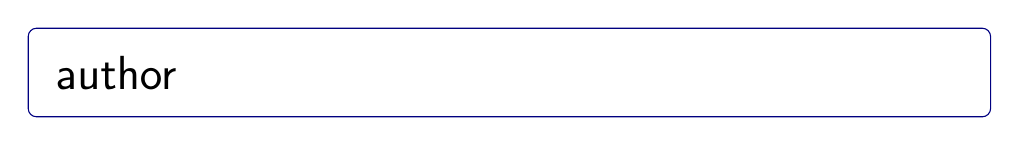
\begin{tikzpicture}
\node[rectangle,rounded corners=3pt,inner sep=10pt,draw=blue!50!black,text width= 0.95\textwidth] {\LARGE \@author};
\end{tikzpicture}
\end{minipage}
\bigskip\bigskip
}%
\makeatother

% custom section
\usepackage[explicit]{titlesec}
\newcommand*\sectionlabel{}
\titleformat{\section}
  {\gdef\sectionlabel{}
   \normalfont\sffamily\Large\bfseries\scshape}
  {\gdef\sectionlabel{\thesection\ }}{0pt}
  {
\noindent
\begin{tikzpicture}
\node[rectangle,rounded corners=3pt,inner sep=4pt,fill=blue!50!black,text width= 0.95\columnwidth] {\color{white}\sectionlabel#1};
\end{tikzpicture}
  }
\titlespacing*{\section}{0pt}{15pt}{10pt}


% custom footer
\usepackage{fancyhdr}
\makeatletter
\pagestyle{fancy}
\fancyhead{}
\fancyfoot[C]{\footnotesize \textcopyright\ \@date\ \ \@author}
\renewcommand{\headrulewidth}{0pt}
\renewcommand{\footrulewidth}{0pt}
\makeatother


\title{Biol 461 Section 01/14/21}
\author{Reading Papers, Time Constant, Space Constant}
\date{01/15/21}



\begin{document}

\maketitle

\begin{multicols*}{2}


\section*{Reading Papers}

This is by no means an authoritative strategy. This is just a very general outline of the strategy I employ.\\

\begin{itemize}
\setlength\itemsep{.5em}
  \item[1] Read the abstract. Glean the identified knowledge gap, the researchers' approach, and the major findings.
  \item[2] Look at figure 1. This is usually the point where I decide whether or not I'm going to read the paper.
  \item[3] Look at a few more figures.
  \item[4] Read (skim) the intro to get an idea of the researcher's perspective of the history of the field.
  \item[5] Read the main conclusions of the paper
  \item[6] Look at the rest of the figures. If I don't understand any read the corresponding discussion or methods section as relevant.\\
\end{itemize}
Unless I am specifically looking for an experimental protocol or I am entirely unfamiliar with the techniques the researchers used, I rarely read the methods section.

\section*{Length Constant}
 $$\lambda = \sqrt{\frac{dR_m}{4R_i}}$$
\begin{itemize}
\setlength\itemsep{.5em}
\item d is the diameter of the neuron
  \item $R_m$ is the resistance of the membrane (across the membrane)
  \item $R_i$ is the resistance of the intracellular matrix
\end{itemize}

The Length Constant is expressed in units of length. One length constant corresponds to the distance at which the peak magnitude of the membrane potential change has attenuated to $\frac{1}{e}$, or about 37\% of the original peak magnitude.

\vfill\null
\columnbreak 
\section*{Time Constant}

$$\tau = R_mC_m$$
\begin{itemize}
\setlength\itemsep{.5em}
  \item $R_m$ is the membrane resistance (across the membrane)
  \item $C_m$ is the membrane capacitance
\end{itemize}
The time constant is expressed in units of time. It is used to describe the rise and fall of membrane voltage. The rise of membrane voltage is described by the equation: 
$$V(t) = V_{max}(1-e^{\frac{-t}{\tau}})$$

$V_{max}$ is the maximum voltage change from resting potential. Setting $t = \tau$ sets $V(t) = 0.63V_{max}$, so after one time constant has passed 63\% of $V_{max}$ as been reached.

\section*{Practice Questions}
\begin{enumerate}
  \item 
  \begin{enumerate} This problem is using the same model cell we described last week.
     \item(a) The resting membrane potential of model cell is -60mV. Using voltage clamp, I change the membrane voltage to 30mV. What will the membrane potential be one time constant past the voltage change? %-3.3mV\\
     \item(b) At t= 22ms the membrane voltage is 20mV. What is the time constant of this cell?
     \end{enumerate}
    \item The squid giant axon can be up to 1.5mm in diameter. Most axons in the human body are about 1uM in diameter. How much further will a membrane potential change passively propagate in the giant squid axon vs the human axon? %39 x further
\end{enumerate}

\end{multicols*}

\end{document}
